% skype+baby monitor
% beamer+notebook
% esp+abs: both control brakes and motor
\subsection{Examples for Feature Interactions}

\begin{frame}{A Common Interaction of Toasters}
	\leftandright{
		\only<1|handout:0>{\pic[width=\linewidth]{toast1}}%
		\only<2|handout:0>{\pic[width=\linewidth]{toast2}}%
		\only<3-|handout:1>{\pic[width=\linewidth]{toast3}}%
		\uncover<5->{\myexample{}{\centering no interaction for two toasts (i.e., \emph{$T_1 \pand T_2$} shown) and for no toasts (i.e., $\pnot T_1 \pand \pnot T_2$ not shown)}}
	}{
		\only<4->{\pic[width=\linewidth]{toast4}}%
		\uncover<6->{\myexample{}{\centering unwanted interaction for one toast\\(i.e., \emph{$T_1 \pand \pnot T_2$} shown and  $\pnot T_1 \pand T_2$ not shown)}}
	}
\end{frame}

\begin{frame}{An Interaction when Customizing Clothes}
	\begin{mycolumns}[widths={66}]
		\includegraphics[width=\linewidth,page=14,trim=30 35 210 105,clip]{2021/2021-09-08-SPLC-Keynote}
	\mynextcolumn
		\begin{example}{Customization of Clothes}
			\begin{itemize}
			\item platforms such as Spreadshirt
			\item store preselects clothes with certain colors
			\item customization with pictures in different colors
			\item where is the problem?
			\end{itemize}
		\end{example}
	\end{mycolumns}
\end{frame}
\begin{frame}{An Interaction when Customizing Clothes}
	\begin{mycolumns}%[widths={40,40}]
		\myexampletight{The Problem: Unwanted Interaction of Colors}{\centering\includegraphics[width=.9\linewidth,page=15,trim=70 35 385 105,clip]{2021/2021-09-08-SPLC-Keynote}}
	\mynextcolumn
		\myexampletight{The Solution: Choose Other Colors}{\centering\includegraphics[width=.9\linewidth,page=15,trim=385 35 70 105,clip]{2021/2021-09-08-SPLC-Keynote}}
	\end{mycolumns}
\end{frame}
\begin{frame}{An Interaction when Customizing Clothes}
	\begin{mycolumns}
		\myexampletight{The Problem: Unwanted Interaction of Colors}{\centering\includegraphics[width=\linewidth,page=16,trim=50 60 360 130,clip]{2021/2021-09-08-SPLC-Keynote}}
	\mynextcolumn
		\myexampletight{The Solution: Choose Other Colors}{\centering\includegraphics[width=\linewidth,page=16,trim=360 60 50 130,clip]{2021/2021-09-08-SPLC-Keynote}}
	\end{mycolumns}
	\uncover<3->{\begin{note}{}
		\centering seems that contrast is checked for each order (i.e., in application engineering)\\and not for each published design (i.e., in domain engineering)
	\end{note}}
\end{frame}

\begin{frame}{An Interaction of Android Apps}
	\begin{mycolumns}[widths={67},animation=none]
		\only<1-2|handout:0>{\includegraphics[width=\linewidth,page=11,trim=40 30 280 100,clip]{2021/2021-09-08-SPLC-Keynote}}%
		\only<3->{\includegraphics[width=\linewidth,page=11,trim=40 30 40 100,clip]{2021/2021-09-08-SPLC-Keynote}}%
		\only<4->{\begin{note}{}%
			\centering which of those 3.5 million Android apps interact?\\where to document?\\whom to blame?%
		\end{note}}%
	\mynextcolumn
		\begin{example}{Skype vs BabyMonitor}
			\begin{itemize}
			\item Skype app installed and used for years
			\item BabyMonitor installed, carefully tried and used for months
			\item BabyMonitor can call any other number (i.e., works without internet)
			\item automatic update of the Skype app
			\item update causes a question to be asked for every call
			\item \alt<-2>{what is the problem?}{found baby crying as no one answered the dialog}
			\end{itemize}
		\end{example}
	\end{mycolumns}
\end{frame}

%\begin{frame}{Can We Trust Our Scans?}
%	\centering\includegraphics[width=\linewidth,page=28,trim=40 30 40 70,clip]{2021/2021-09-08-SPLC-Keynote}
%\end{frame}
% TODO add scanner example? is it really dependent on multiple options? or only on one particular setting

\begin{frame}{Known Interactions of Lenovo Hardware}
	\centering\includegraphics[height=\textheightwithtitle,page=19]{2021/2021-09-08-SPLC-Keynote}
\end{frame}
\begin{frame}{Known Interactions of Lenovo Hardware}
	\centering\includegraphics[height=\textheightwithtitle,page=20]{2021/2021-09-08-SPLC-Keynote}
\end{frame}
\begin{frame}{Known Interactions of Lenovo Hardware}
	\centering\includegraphics[height=\textheightwithtitle,page=21]{2021/2021-09-08-SPLC-Keynote}
\end{frame}
\begin{frame}
	\centering\includegraphics[width=\linewidth,page=22,trim=40 20 40 0,clip]{2021/2021-09-08-SPLC-Keynote}
\end{frame}

\subsection{Static and Dynamic Interactions}
\begin{frame}{Interactions with Preprocessors}
	\centering
	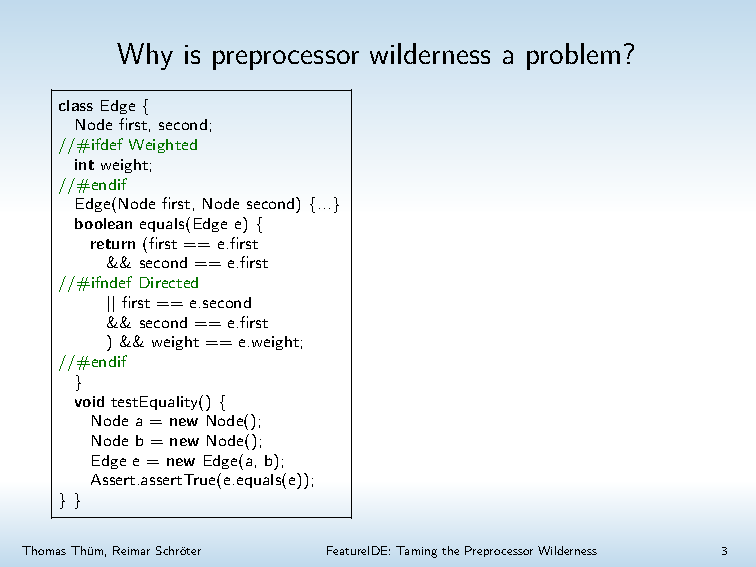
\includegraphics[height=\textheightwithtitle,page=1,trim=20 20 20 40,clip]{preprocessor-wilderness}
\end{frame}
\begin{frame}{No Interaction}
	\centering
	\includegraphics[height=\textheightwithtitle,page=2,trim=20 20 20 40,clip]{preprocessor-wilderness}
\end{frame}
\begin{frame}{A Static Interaction}
	\centering
	\includegraphics[height=\textheightwithtitle,page=3,trim=20 20 20 40,clip]{preprocessor-wilderness}
\end{frame}
\begin{frame}{Another Static Interaction}
	\centering
	\includegraphics[height=\textheightwithtitle,page=4,trim=20 20 20 40,clip]{preprocessor-wilderness}
\end{frame}
\begin{frame}{A Dynamic Interaction}
	\centering
	\includegraphics[height=\textheightwithtitle,page=5,trim=20 20 20 40,clip]{preprocessor-wilderness}
\end{frame}

\subsection{Unwanted and Wanted Interactions} % Desired + Undesired
% \href{https://github.com/SoftVarE-Group/Slides/blob/main/2021/2021-09-08-SPLC-Keynote.pdf}{\mycite{Every unwanted feature interaction waits to be fixed or at least documented in form of a constraint.}} T:SPLC21 

\subsection{Pairwise Interactions}
\subsection{Higher-Order Interactions}

\begin{frame}{Interaction on Data and Control Flow \mytitlesource{\essentialconfigurationcomplexity}}
	\centering
	\essentialconfigurationcomplexitylink{\includegraphics[height=\textheightwithtitle,page=2,trim=55 495 225 75,clip]{2016/2016-ASE-Meinicke}}
\end{frame}
\begin{frame}{Execution Traces in Configurable Systems \mytitlesource{\essentialconfigurationcomplexity}}
	\essentialconfigurationcomplexitylink{\includegraphics[width=\linewidth,page=8,trim=55 520 55 55,clip]{2016/2016-ASE-Meinicke}}
\end{frame}

% example from the The Variability Bug Database

% TODO explain duality between partial configurations and conjunctions of literals (cf. elevator product line by Varshosaz et al.)

